\section{Injustice gods among us}

\begin{figure}[htbp]
\begin{center}
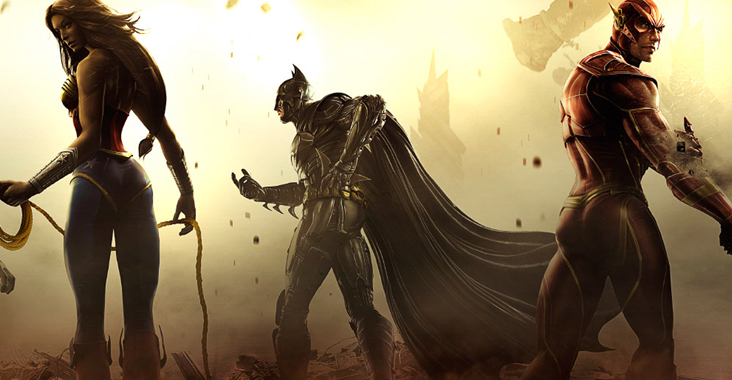
\includegraphics[width=.60\textwidth]{./imagenes/InjusticeGame.jpg}
\caption{Injustice: gods among us}
\label{Injustice: Gods Amoung us}
\end{center}
\end{figure}
Injustice\footnote{Kevin Campuzano}:Injustice \footnote{\url{https://www.injustice.com/en}} Es un juego desarrollado por Warner Brothers Games y es multiplataforma. Es un juego donde todos se enfrentan contra todos, ya sea villano o heroe, tienes la oportunidad de escoger a 3 de ellos y a medida que se va avanzado en el juego se desbloquean nuevos jugadores.

Cada heroe o villano tiene habilidades especiales que se recargan con medida de que se pelea.

\subsubsection{¿Por qué es uno de mis juegos favoritos?}
\begin{itemize}
	\item La grafica del juego es muy opinion es Excelente.
	\item Es el juego que mas tiempo llevo jugando en mi ipad recientemente comprado.
	\item No conocia de ciertos villanos hasta el momento en que lo jugue.
	\item Hay tantos personas y la mayoria de ellos tiene su perfil de insurgencia y regimen.
	\item Los personajes en mi poder en este momento son:
		\begin{itemize}
			\item Flash
			\item Flecha Verde.
			\item Lex Luthor.
			\item Gatubela(Esa vino por Default).
			\item Siniestro.
			\item Nightwing(Robin).
		\end{itemize}	
\end{itemize}